\section{Simulation Analysis}
\label{sec:simulation}

\subsection{Transient analysis}

We simulated the circuit using transient and frequency analysis, using the supplied model of transistors:

\begin{table}[H]
\addtolength{\tabcolsep}{-4pt}
\caption{Values of capacitances and resistances for various circuit components}
\vspace{-3mm}
\begin{tabular}{|c|c|c|}
\hline\\
Vc & 12.0 V\\
Vs & 10e-3 V\\
Rs & 100 Ohm\\
Ci & 1e-3 F\\
Rb1& 80e3 Ohm\\
Rb2 &20e3 Ohm\\
Rc & 1e3 Ohm\\
Re &100 Ohm\\
Ce & 1e-3 F\\
Von&0.7 V\\
Vt&25e-3 V\\
Va1&69.7 V\\
Va2&37.2 V\\
Rd & 100 Ohm\\
Co & 1e-6 F\\
Rl & 8 Ohm\\
\hline
\end{tabular}
\label{tab:Components}
\end{table}

\par

Firstly, we performed an operating point analysis, some of the relevant results obtained are below:

\begin{table}[H]
    \addtolength{\tabcolsep}{-4pt}
    \caption{OP simulation}
    \vspace{-3mm}
    \begin{tabular}{|c|c|}
    \hline\\
    $I_{e1}$ & $8.72642e-03$\\
    $I_{c1}$ & $8.675224e-03$\\
    $I_{b1}$ & $5.119304e-05$\\  
    $V_{CE1}$ & $3.0214713$\\
    $I_{e2}$ & $7.29143e-02$\\
    $I_{c2}$ & $7.234499e-02$\\
    $I_{b2}$ & $5.693370e-04$\\  
    $V_{CE2}$ & $4.708568$\\
    \hline
    \end{tabular}
    \label{tab:OP_sim}
\end{table}

Using transient analysis, and frequency f=1e3 Hz, we simulate the circuit, which yields the following $v_7(t)$:

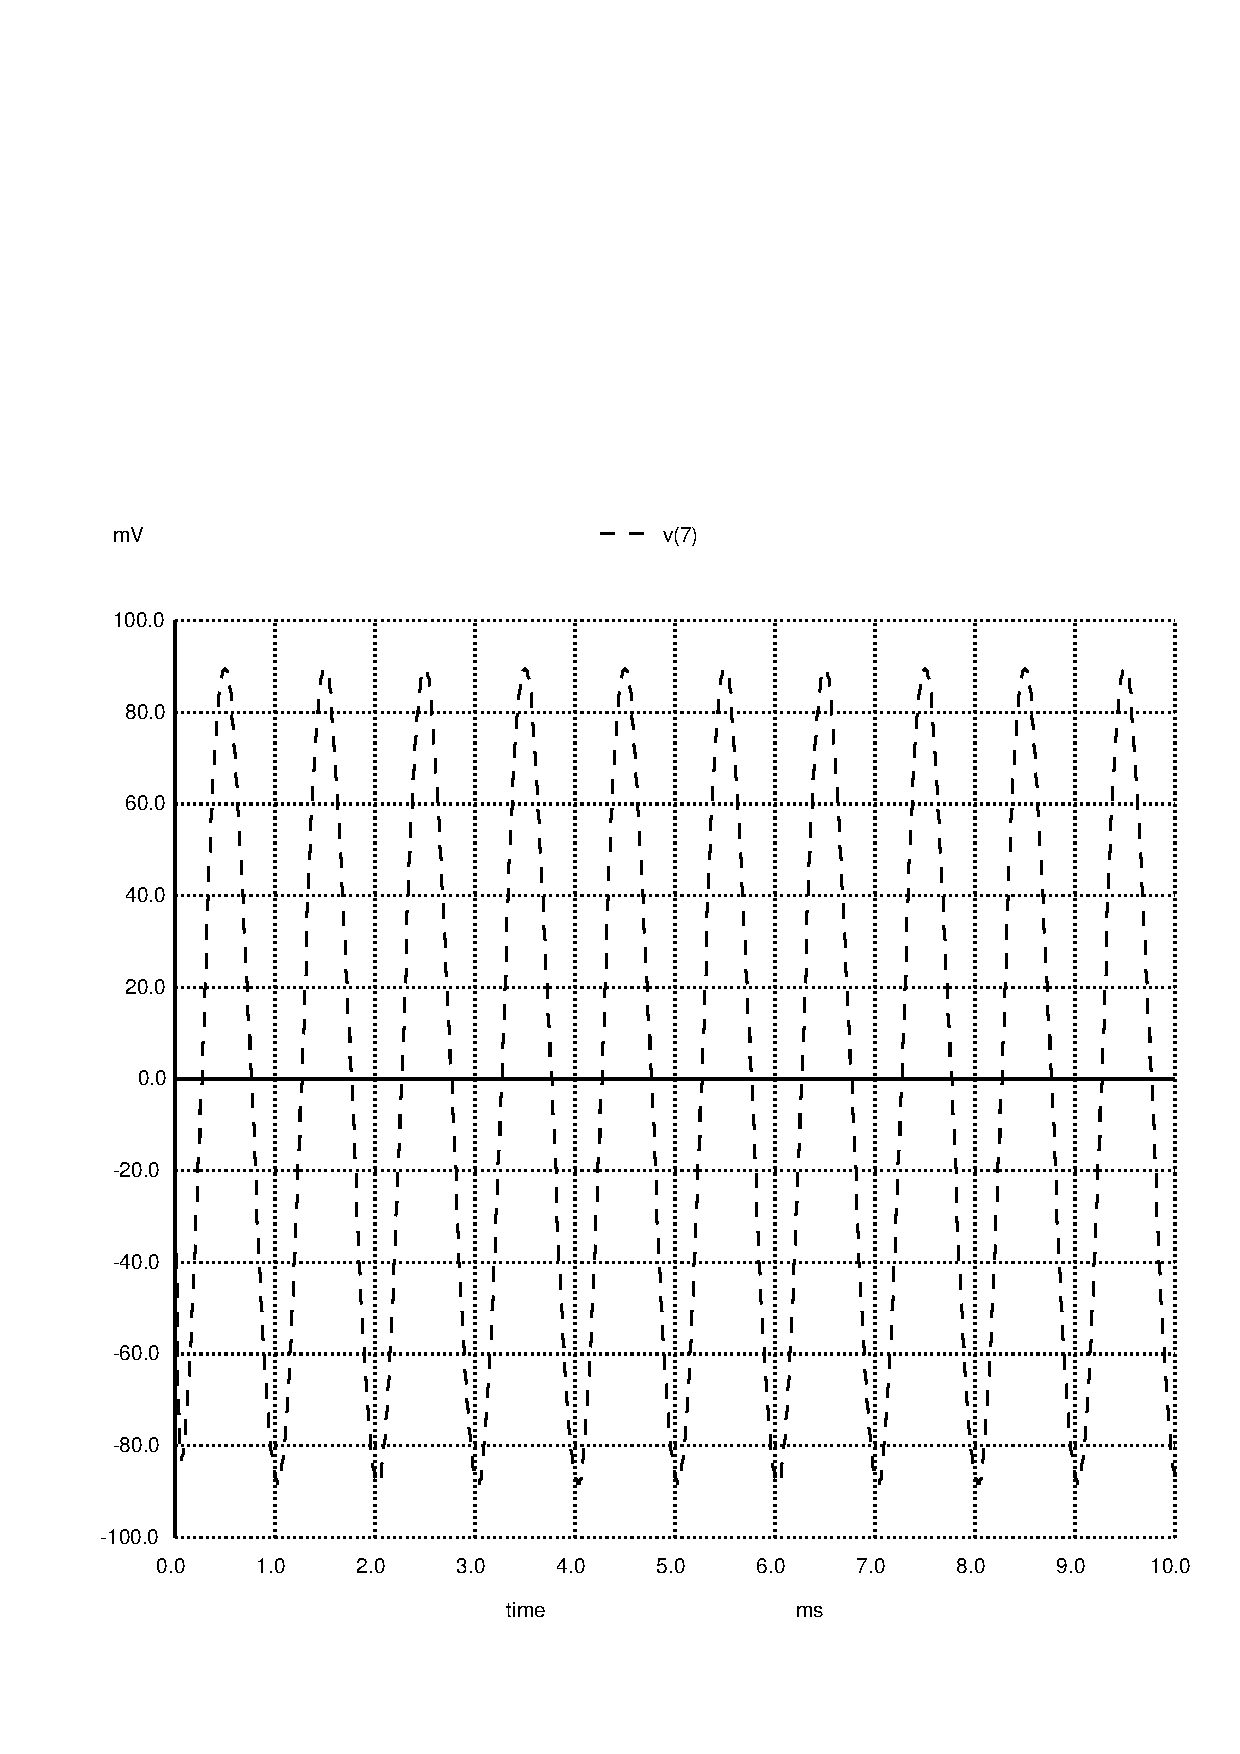
\includegraphics[width=0.8\linewidth]{../sim/vo1.pdf}

We simulate the circuit using frequency analysis and max(vs(t))=1, obtaining the following gain in $v_2$, which is the gain after the gain stage:

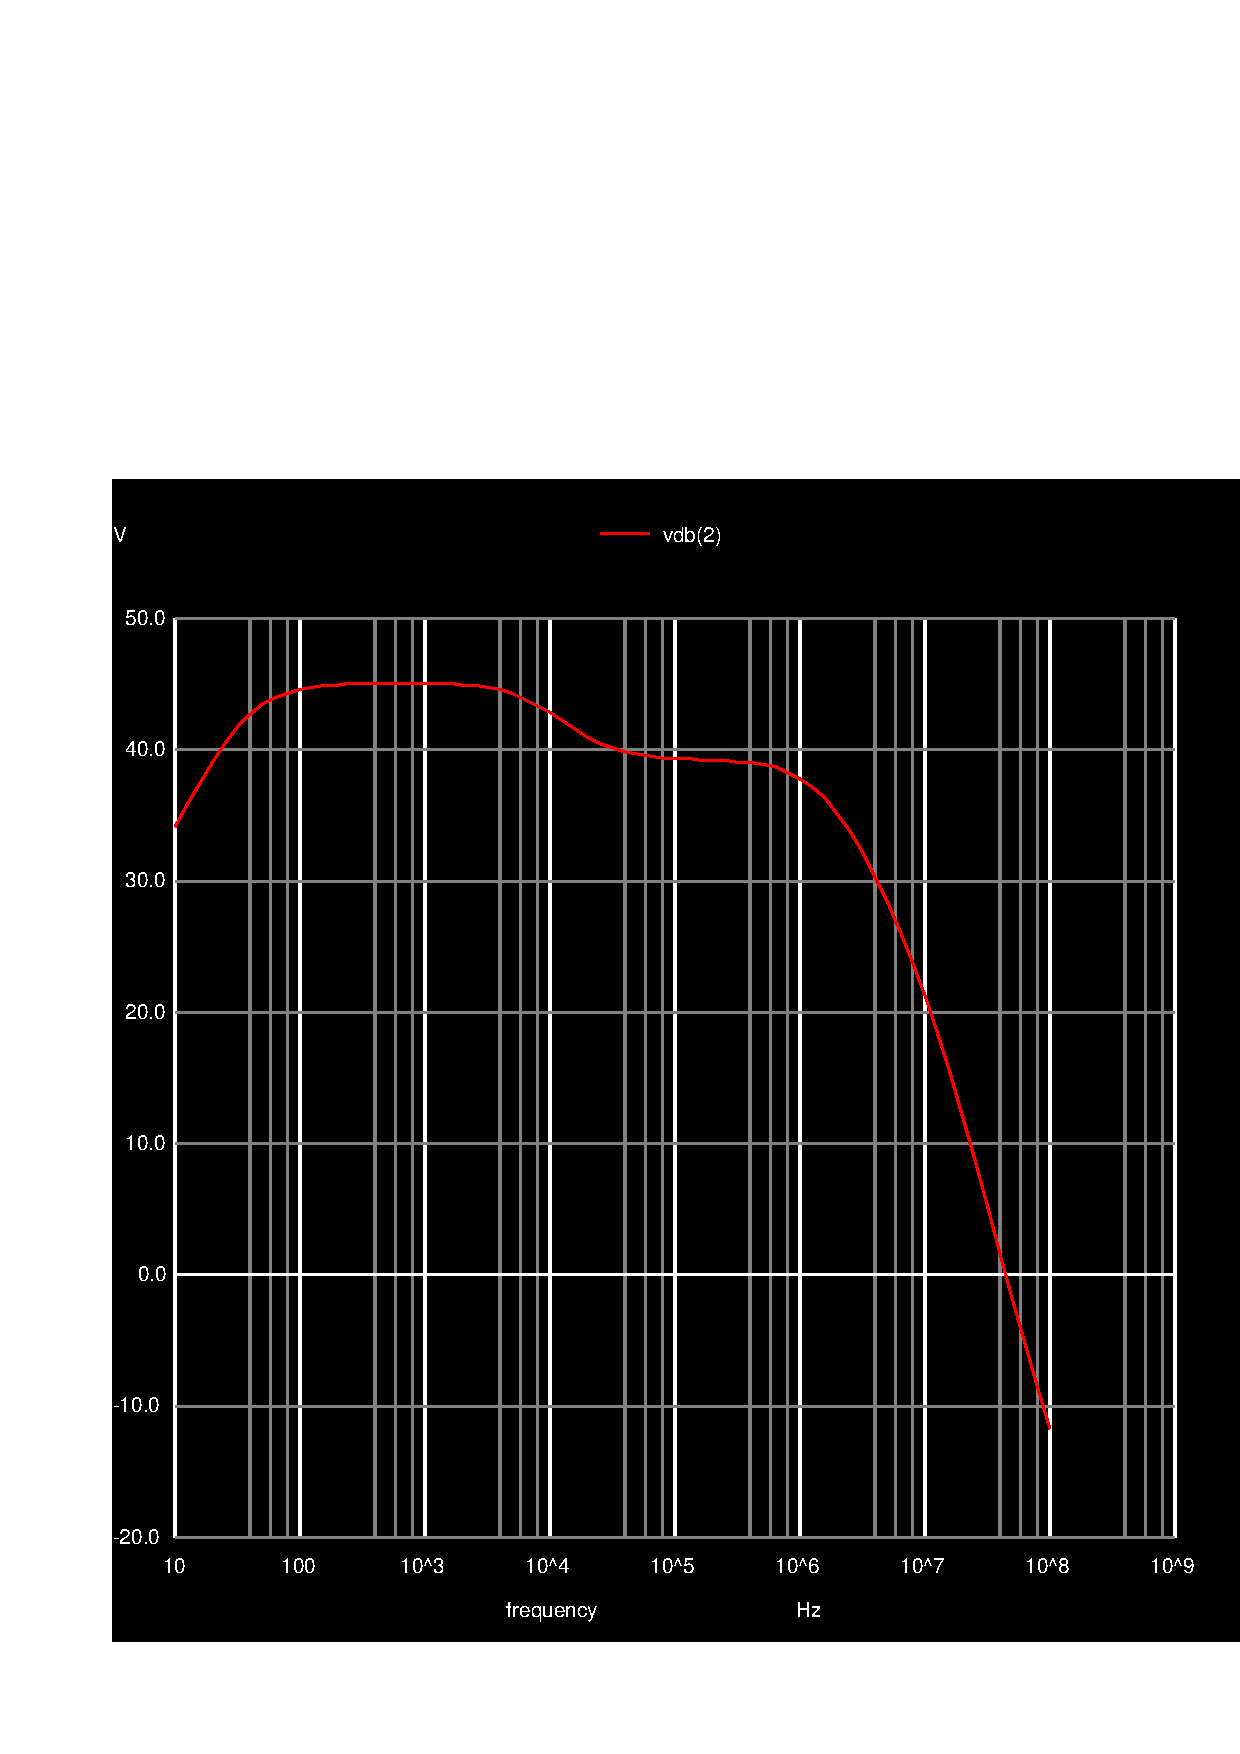
\includegraphics[width=0.8\linewidth]{../sim/vo1f.pdf}

And the gain in $v_7$,which is the gain after the output stage:

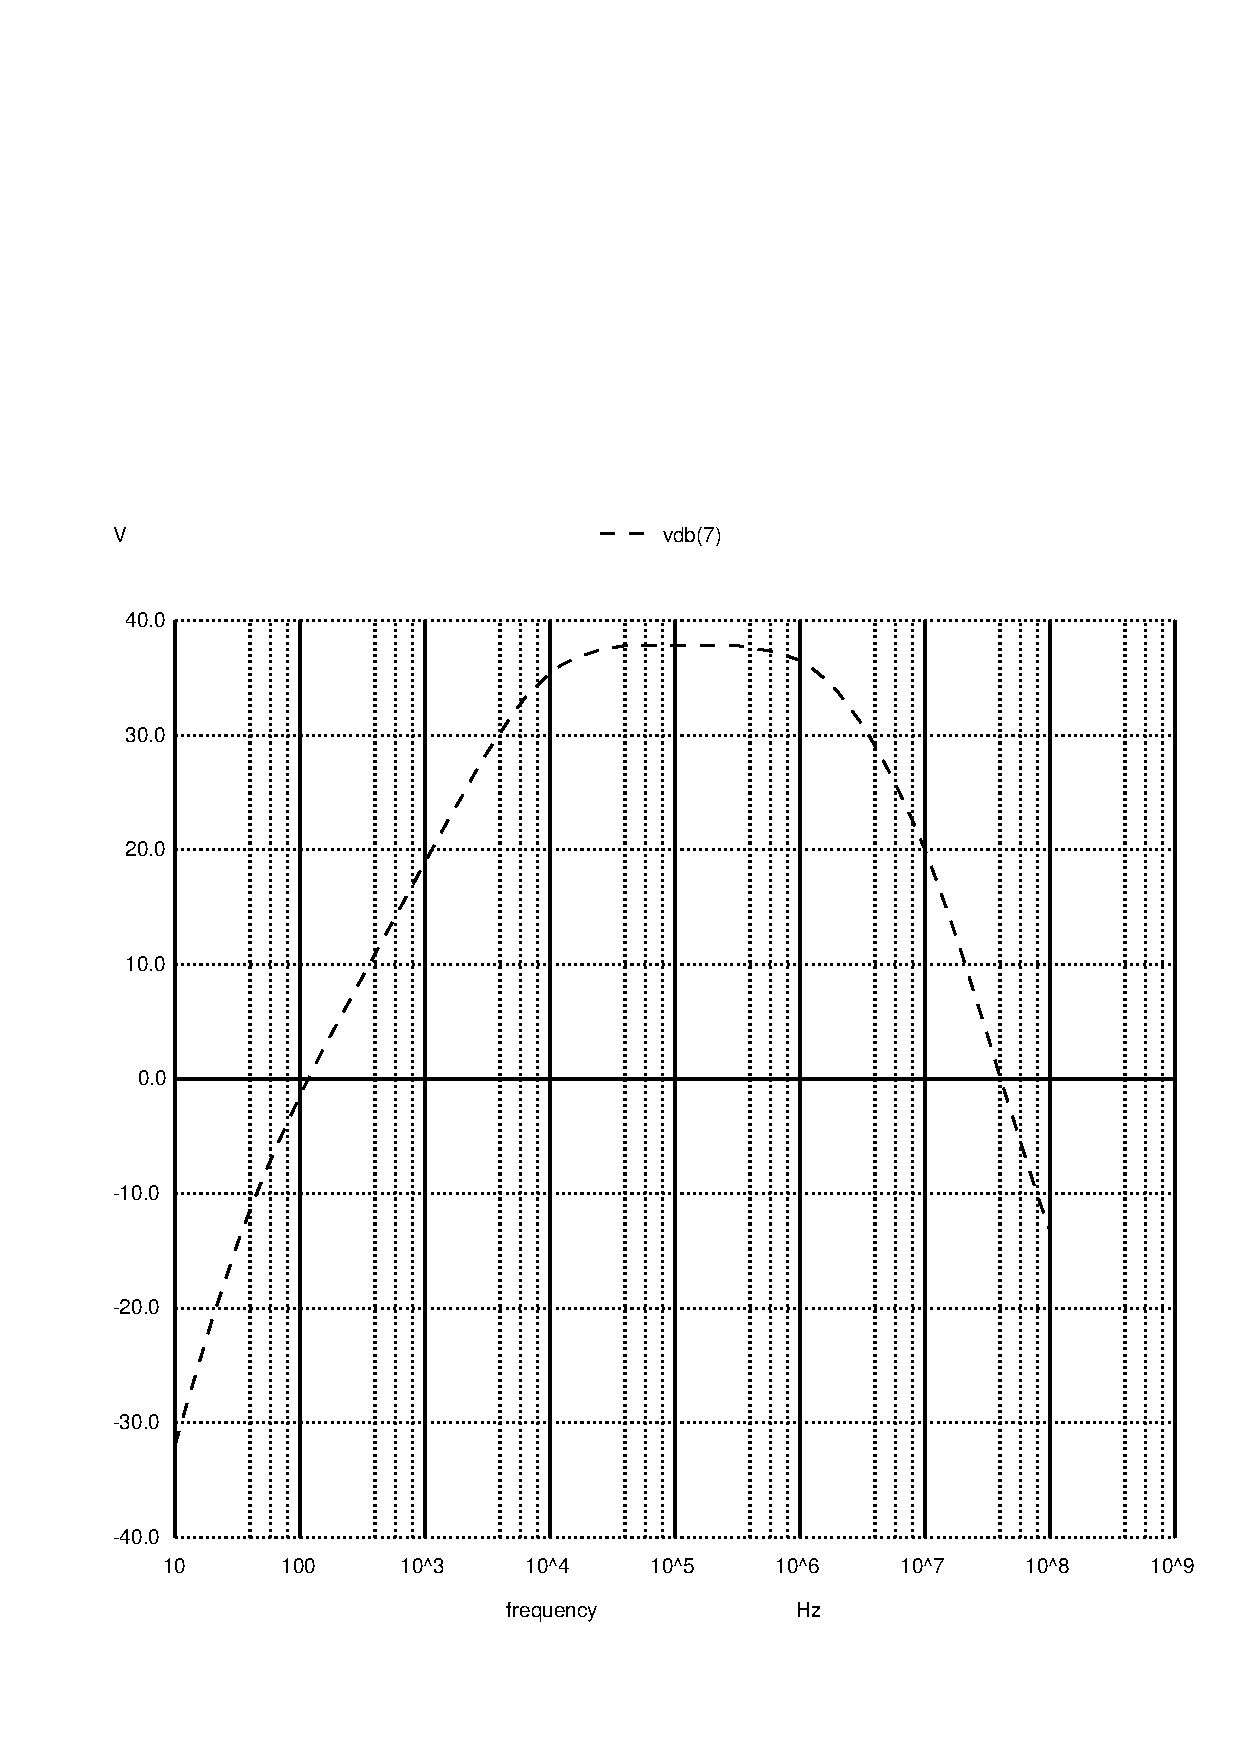
\includegraphics[width=0.8\linewidth]{../sim/vo2f.pdf}

\par


This circuit has a cost of 2102.508, voltage gain 3.790425e+01, bandwidth 1.594837e+06, minimum voltage cuttoff 8.880395e+03 and the  calculated Merit is 3.238.